% \subsection{Pengujian Citra \emph{Depth Camera} di Simulasi}
% \label{subsec:citradepthsimulasi}

\begin{figure}[ht]
  \centering
  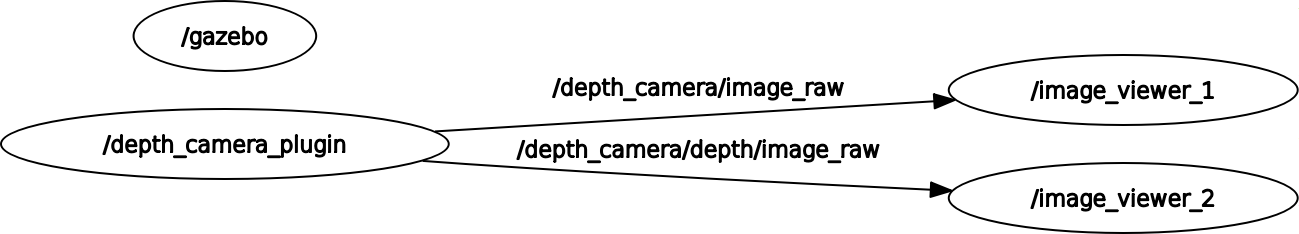
\includegraphics[width=0.95\textwidth,keepaspectratio]{gambar/rosgraph-depth-camera-plugin.png}
  \caption{Relasi antar-\emph{node} dari pengujian citra \emph{depth camera} di simulasi.}
  \label{fig:rosgraphdepthcameraplugin}
\end{figure}

% \textcolor{red}{\lipsum[1-2]}

\begin{figure}[ht]
  \centering
  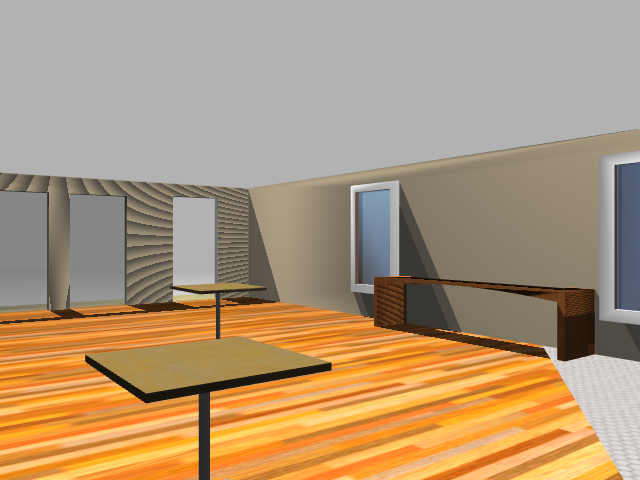
\includegraphics[width=0.45\textwidth,keepaspectratio]{gambar/citra-depth-camera-rgb-simulasi.png}
  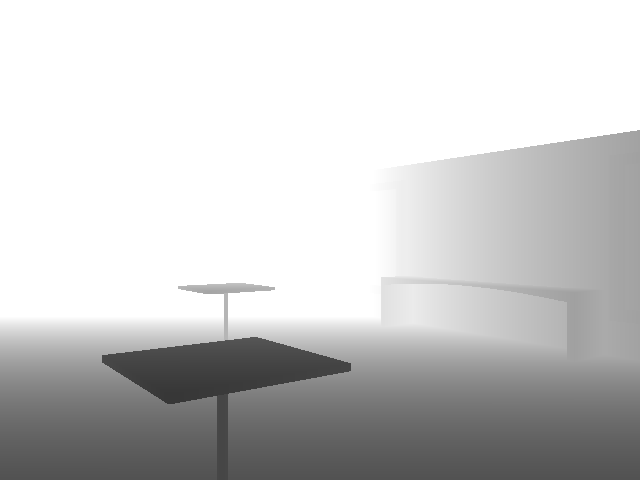
\includegraphics[width=0.45\textwidth,keepaspectratio]{gambar/citra-depth-camera-depth-simulasi.png}
  \caption{Perbandingan hasil tangkapan citra berwarna dan citra kedalaman di simulasi.}
  \label{fig:depthcamerasimulasi}
\end{figure}
